% ============================================================
% M2 轮4 S3 · 练习件 第5课时（§1.1.3 课2 空间向量运算的坐标表示）
% 题面：照题面库 成卷/题面库/课时05-1.1.3课2.md 全 16 题冻结入卷（卷面题号＝库序 1~16）；
%       组名/难度照库头第 3/4 字段（组名批替换后正名照录：第15/16题＝「存在性判定×值域」「双动点定距×数量积范围」新组名）。
%       第5/6题库头组名标「×填空」但题面为单选/解答→照题面形制排版，登记。
%       第14题「平行六面体ABCD-ABC₁D₁」记号脱字按亲算-1.1.3-a T9·纠错6(a) 规范化为 ABCD-A₁B₁C₁D₁（改字不改果，落台账）。
% 模板基线＝练习线样张（六宏零改动拷入）；版式＝练习线 p2 课时训练
%       （\keshi＋multicols＋花形三档 基础巩固1~10／综合提升11~14／思维探索15~16）。
% 图源：第12题＝讲上 image11.png→js_image11.png(45mm，T7 正方体图，与导学件课时05 图同源逐字节 cmp 一致)；
%       第14题＝讲上 image12.png→js_image12.png(58mm，T9 斜60°平行六面体图，同前)。
% 取值/组名照登对照/图位/登记事项：见 ../批2值台账.md 课时05 节。
% 编译：xelatex main.tex（两遍）→ python render.py → png/pageN.png
% ============================================================
\documentclass[fontset=none]{ctexart}
\usepackage{qp-m3} % 换装：六宏→qp-m3 单包（钉后版 md5 7c3930362be8a0a2bdf21bbf8ac16573，两补钉随版）

% ============================================================
% 练习件局部宏（照练习线样张页2形制搬入；本段只加件，不改件）
% ============================================================
\renewcommand{\qpjianming}{练习件}
\renewcommand{\qpceming}{高中数学\quad 选择性必修第一册(人教B版)} % 换装回钉：qp-m3 默认册名＝选必二，防页脚漂移（试迁规约·试迁报告§四 B3 实证必改）
\renewcommand{\qpzhangming}{第一章\quad 空间向量与立体几何}

% ---------- YJ-01 灰块页脚·练习册档（块 31.0×7.8mm，照练习线样张 31.0mm 修正版） ----------
\newcommand{\qpxsyema}{\ifnum\value{page}<10 00\fi\ifnum\value{page}>9 \ifnum\value{page}<100 0\fi\fi\arabic{page}}
\newcommand{\lxshuziL}{\hbox to 13.8mm{\setlength{\fboxsep}{0pt}\colorbox{pnumbg}{%
  \makebox[31.0mm][l]{\rule[-3.145mm]{0pt}{7.8mm}\hspace{2.8mm}\fontsize{10.7pt}{13pt}\selectfont\color{black}\numpnum\qpxsyema}}\hss}}
\newcommand{\lxshuziR}{\hbox to 13.8mm{\kern-17.2mm\setlength{\fboxsep}{0pt}\colorbox{pnumbg}{%
  \makebox[31.0mm][r]{\rule[-3.145mm]{0pt}{7.8mm}\fontsize{10.7pt}{13pt}\selectfont\color{black}\numpnum\qpxsyema\hspace{2.75mm}}}}}
\fancyfoot[RO]{\raisebox{-1.24mm}[0pt][0pt]{\qphuitext\qpzhangming\quad{\heiti\qpjianming}\hspace{3mm}\lxshuziL}}
\fancyfoot[LE]{\raisebox{-1.24mm}[0pt][0pt]{\lxshuziR\hspace{3mm}\qphuitext\qpceming}}

% ---------- HX-01 花形·三档名（练习册版 25.5×6.8mm，重叠 o＝5.1mm，照练习线样张裁定值） ----------
% 局部宏 \huadianOverlapLx 已由 qp-m3 收编（等值定义），依换装方案§1.4 预删防撞名
% 局部宏 \dangbadge 已由 qp-m3 收编（等值定义），依换装方案§1.4 预删防撞名

% ---------- TJ-02 练习册悬挂题号（单号 5.75mm／双位 7.6mm，题号 \textbf 加重） ----------
% 长度 \lxhang 已由 qp-m3 分配，预删防重复定义
% 局部宏 \tihao 已由 qp-m3 收编（等值定义），依换装方案§1.4 预删防撞名
% 选项段（TJ-07 行距档；左缘随题号悬挂）
% 局部宏 \lxopt 已由 qp-m3 收编（等值定义），依换装方案§1.4 预删防撞名
% 解答题书写位留白
% 局部宏 \xiexwei 已由 qp-m3 收编（等值定义），依换装方案§1.4 预删防撞名
% 组名栏宏（组名照题面库头第 3 字段照登，去〔代表〕〔第N题〕簿记标）
% 局部宏 \zu 已由 qp-m3 收编（等值定义），依换装方案§1.4 预删防撞名

\begin{document}

% ============================================================
% 课时训练（三档 10＋4＋2＝16 题）
% ============================================================
\keshi{第5课时\quad 空间向量运算的坐标表示}
\begin{multicols}{2}
\emergencystretch=1em

\dangbadge{基}{础}{巩}{固}

\tihao{1}\zu{det 平行判定题组（坐标）×判断} \tieside{简单}分别判断下列各对向量是否平行：
\lxopt{(1)\((0,0,5)\)与\((0,0,7)\)；}
\lxopt{(2)\((4,0,3)\)与\((8,0,6)\)．}
\xiexwei{16mm}
\begin{ansblock}[练-课时05-1]
% ans:练-课时05-1
\ansitem{1}{(1)(2) 均平行}
\end{ansblock}

\tihao{2}\zu{det 垂直判定} \tieside{简单}分别判断下列各对向量是否垂直：
\lxopt{(1)\((3,4,0)\)与\((0,0,5)\)；}
\lxopt{(2)\((3,1,3)\)与\((1,0,-1)\)．}
\xiexwei{16mm}
\begin{ansblock}[练-课时05-2]
% ans:练-课时05-2
\ansitem{2}{(1)(2) 均垂直}
\end{ansblock}

\tihao{3}\zu{moddir 平行＋模长反求坐标×填空} \tieside{简单}若\(\overrightarrow{a}=(1,-1,2)\)，向量\(\overrightarrow{AB}\)与\(\overrightarrow{a}\)平行且\(|\overrightarrow{AB}|=2\sqrt{6}\)，则\nobreak\(\overrightarrow{AB}=\)\kongbai{}．
\begin{ansblock}[练-课时05-3]
% ans:练-课时05-3
\ansitem{3}{\((2,-2,4)\) 或 \((-2,2,-4)\)}
\end{ansblock}

\tihao{4}\zu{c3b 线段上定比分点坐标×填空} \tieside{简单}若\(A(3,2,4)\)，\(B(1,2,-8)\)，点\(C\)在线段\(AB\)上，且\(\frac{|AC|}{|AB|}=\frac{2}{3}\)，则点\(C\)的坐标是\kongbai{}．
\begin{ansblock}[练-课时05-4]
% ans:练-课时05-4
\ansitem{4}{C\(\left(\dfrac{5}{3},2,-4\right)\)}
\end{ansblock}

\tihao{5}\zu{c5 平行四边形已知三顶点求第四顶点×填空} \tieside{简单}若四边形\(ABCD\)是平行四边形，且\(A(4,1,3)\)，\(B(2,-5,1)\)，\(C(3,7,-5)\)，则顶点\(D\)的坐标为\nobreak(\kongwei)
\lxopt{\makebox[\dimexpr0.5\linewidth-0.5\lxhang-0.25em\relax][l]{A．\((1,1,-7)\)；}\makebox[\dimexpr0.5\linewidth-0.5\lxhang-0.25em\relax][l]{B．\((5,3,1)\)}}
\lxopt{\makebox[\dimexpr0.5\linewidth-0.5\lxhang-0.25em\relax][l]{C．\((-3,1,5)\)；}\makebox[\dimexpr0.5\linewidth-0.5\lxhang-0.25em\relax][l]{D．\((5,13,-3)\)}}
\begin{ansblock}[练-课时05-5]
% ans:练-课时05-5
\ansitem{5}{D\((5,13,-3)\)}
\end{ansblock}

\tihao{6}\zu{par2 组合向量平行求单参 m×填空} \tieside{简单}已知\(\overrightarrow{a}=(-2,3,2)\)，\(\overrightarrow{b}=(1,-5,1)\)，且\(m\overrightarrow{a}+\overrightarrow{b}\)与\(2\overrightarrow{a}-\overrightarrow{b}\)平行，求实数\(m\)的值．
\xiexwei{16mm}
\begin{ansblock}[练-课时05-6]
% ans:练-课时05-6
\ansitem{6}{\(m=-2\)}
\end{ansblock}

\tihao{7}\zu{opmod 模长＋垂直双条件并列定参×单选} \tieside{简单}向量\(\overrightarrow{a}=(2,1,x)\)，\(\overrightarrow{b}=(2,y,-1)\)，若\(|\overrightarrow{a}|=\sqrt{5}\)，且\(\overrightarrow{a}\perp\overrightarrow{b}\)，则\nobreak\(x+y\)的值为\nobreak(\kongwei)
\lxopt{\makebox[\dimexpr0.25\linewidth-0.25\lxhang-0.25em\relax][l]{A．\(-1\)；}\makebox[\dimexpr0.25\linewidth-0.25\lxhang-0.25em\relax][l]{B．\(1\)；}\makebox[\dimexpr0.25\linewidth-0.25\lxhang-0.25em\relax][l]{C．\(-4\)；}\makebox[\dimexpr0.25\linewidth-0.25\lxhang-0.25em\relax][l]{D．\(4\)}}
\begin{ansblock}[练-课时05-7]
% ans:练-课时05-7
\ansitem{7}{C（\(-4\)）}
\end{ansblock}

\tihao{8}\zu{angle1 夹角余弦坐标式×题组} \tieside{简单}求下列两个空间向量夹角的余弦：
\lxopt{(1)\(\overrightarrow{a}=(2,-3,\sqrt{3})\)，\(\overrightarrow{b}=(1,0,0)\)；}
\lxopt{(2)\(\overrightarrow{a}=(-1,-1,1)\)，\(\overrightarrow{b}=(-1,0,1)\)．}
\xiexwei{16mm}
\begin{ansblock}[练-课时05-8]
% ans:练-课时05-8
\ansitem{8}{(1)\(\dfrac{1}{2}\)；(2)\(\dfrac{\sqrt{6}}{3}\)}
\end{ansblock}

\tihao{9}\zu{perp-seed 求同时垂直两向量的向量×解答} \tieside{简单}已知向量\(\overrightarrow{a}=(1,0,-1)\)，\(\overrightarrow{b}=(0,1,-1)\)，求一个空间向量\(\overrightarrow{n}\)，使\(\overrightarrow{n}\perp\overrightarrow{a}\)且\(\overrightarrow{n}\perp\overrightarrow{b}\)．
\xiexwei{16mm}
\begin{ansblock}[练-课时05-9]
% ans:练-课时05-9
\ansitem{9}{\(\overrightarrow{n}=\lambda(1,1,1)\)（\(\lambda\neq 0\)）}
\end{ansblock}

\tihao{10}\zu{proj 投影数量（坐标式）×填空} \tieside{简单}已知\(A(0,0,0)\)，\(B(2,5,0)\)，\(C(1,3,5)\)，求\(\overrightarrow{AC}\)在\(\overrightarrow{AB}\)上投影的数量．
\xiexwei{16mm}
\begin{ansblock}[练-课时05-10]
% ans:练-课时05-10
\setlength{\anshang}{7.6mm}% 题10 起双位档（照答案册同值，块内局部）
\ansitem{10}{\(\dfrac{17\sqrt{29}}{29}\)}
\end{ansblock}

\dangbadge{综}{合}{提}{升}

\tihao{11}\zu{comp 中点坐标＋模＋数量积求参＋夹角余弦×四步链} \tieside{中档}已知点\(A(0,1,2)\)，\(B(1,-1,3)\)，\(C(1,5,-1)\)．
\lxopt{(1)若\(D\)为线段\(BC\)的中点，求线段\(AD\)的长；}
\lxopt{(2)若\(\overrightarrow{AD}=(2,a,1)\)，且\(\overrightarrow{AB}\cdot\overrightarrow{AD}=1\)，求\(a\)的值，并求此时向量\(\overrightarrow{AB}\)与\(\overrightarrow{AD}\)夹角的余弦值．}
\xiexwei{16mm}
\begin{ansblock}[练-课时05-11]
% ans:练-课时05-11
\setlength{\anshang}{7.6mm}% 题11 起双位档（照答案册同值，块内局部）
\ansitem{11}{(1)\(\sqrt{3}\)；(2)\(a=1\)，\(\cos=\dfrac{1}{6}\)}
\end{ansblock}

\tihao{12}\zu{move 正方体系定比分点／轴对称／动点距离最值×三问} \tieside{中档}如图，以棱长为\(1\)的正方体的三条棱所在直线为坐标轴，建立空间直角坐标系\(O\text{-}\penalty100 xyz\)，点\(P\)在线段\(AB\)上，点\(Q\)在线段\(DC\)上．
\par\vspace{1.9mm}\penalty10000\noindent\makebox[\linewidth][c]{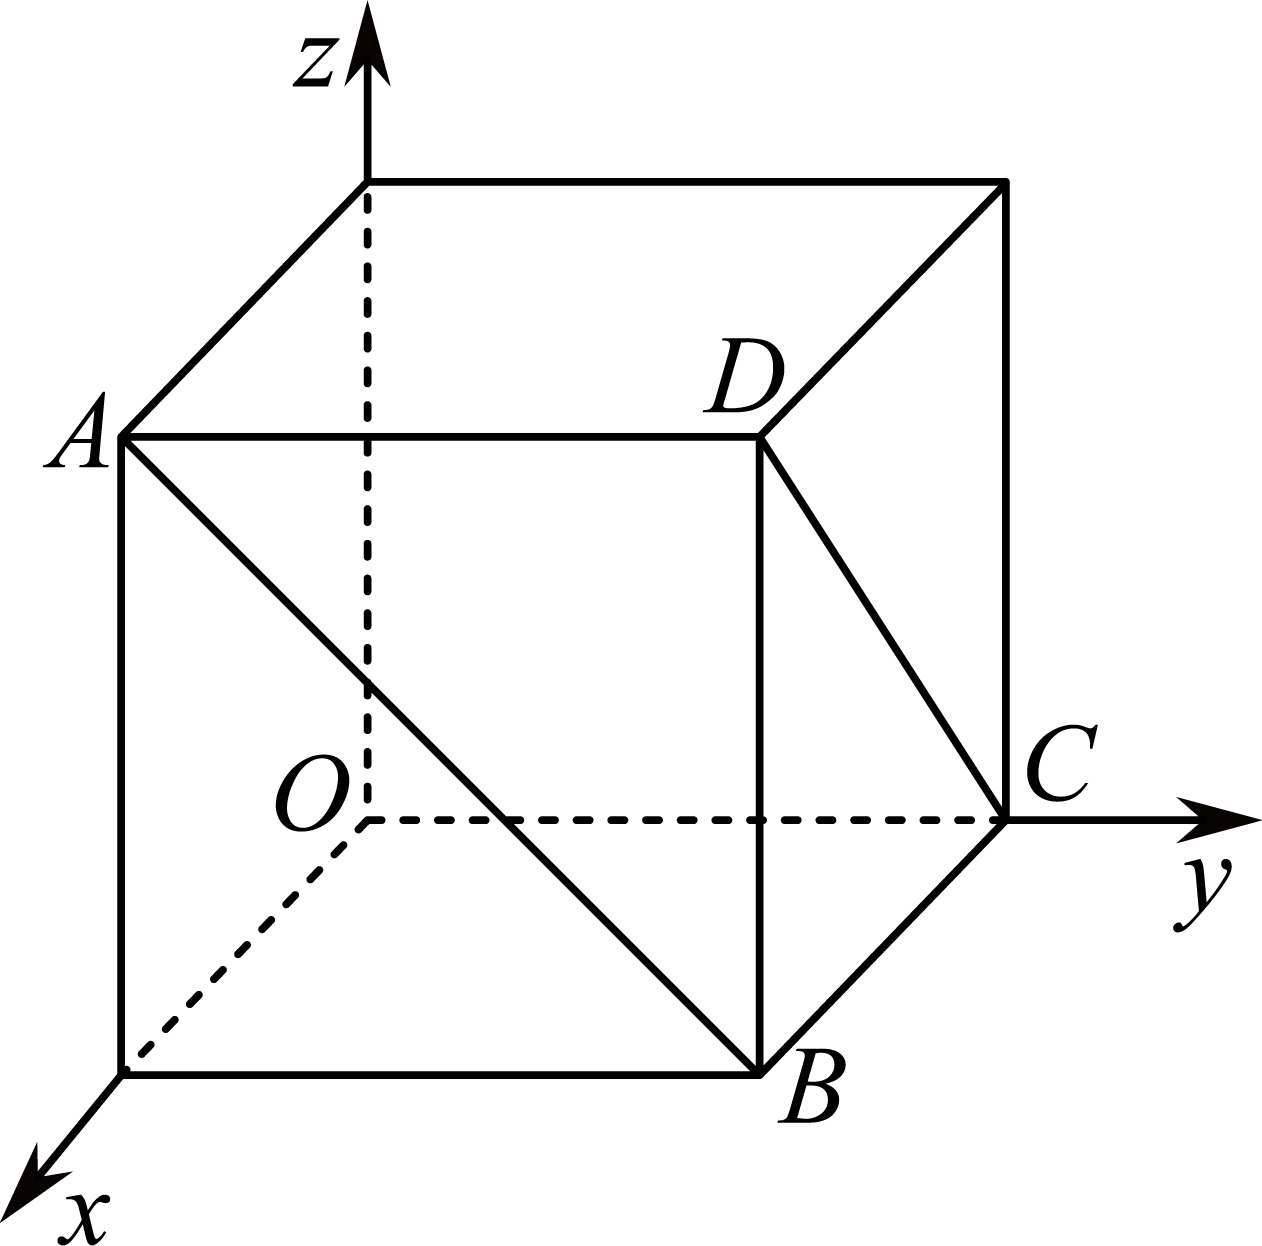
\includegraphics[width=45.0mm]{figs/js_image11.png}}\par\vspace{-1.0mm}\penalty-50
\lxopt{(1)当\(\overrightarrow{PB}=2\overrightarrow{AP}\)，且点\(P\)关于\(y\)轴的对称点为\(M\)时，求\(|PM|\)的长度；}
\lxopt{(2)当点\(P\)是面对角线\(AB\)的中点，点\(Q\)在面对角线\(DC\)上运动时，探究\(|PQ|\)的最小值．}
\xiexwei{16mm}
\begin{ansblock}[练-课时05-12]
% ans:练-课时05-12
\setlength{\anshang}{7.6mm}% 题12 起双位档（照答案册同值，块内局部）
\ansitem{12}{(1)\(\dfrac{2\sqrt{13}}{3}\)；(2)\(\dfrac{\sqrt{6}}{4}\)}
\end{ansblock}

\tihao{13}\zu{par1 平行与垂直坐标条件求参×双问双法} \tieside{中档}已知向量\(\overrightarrow{a}=(2,4,5)\)，\(\overrightarrow{b}=(3,x,y)\)．
\lxopt{(1)若\(\overrightarrow{a}\parallel\overrightarrow{b}\)，求实数\(x\)，\(y\)的值；}
\lxopt{(2)若\(\overrightarrow{a}\perp\overrightarrow{b}\)，且\(|\overrightarrow{b}|=\sqrt{29}\)，求实数\(x\)，\(y\)的值．}
\xiexwei{16mm}
\begin{ansblock}[练-课时05-13]
% ans:练-课时05-13
\setlength{\anshang}{7.6mm}% 题13 起双位档（照答案册同值，块内局部）
\ansitem{13}{(1)\(x=6\)，\(y=\dfrac{15}{2}\)；(2)\((-4,2)\) 或 \(\left(\dfrac{116}{41},-\dfrac{142}{41}\right)\)}
\end{ansblock}

\tihao{14}\zu{newdef 新定义「斜60°坐标系」×解答} \tieside{中档}空间中，两两互相垂直且有公共原点的三条数轴构成直角坐标系，如果坐标系中有两条坐标轴不垂直，那么这样的坐标系称为“斜坐标系”．现有一种空间斜坐标系，它任意两条数轴的夹角均为\(60^{\circ}\)，我们将这种坐标系称为“斜\(60^{\circ}\)坐标系”．我们类比空间直角坐标系，定义“空间斜\(60^{\circ}\)坐标系”下向量的斜\(60^{\circ}\)坐标：\(\overrightarrow{i}\)，\(\overrightarrow{j}\)，\(\overrightarrow{k}\)分别为“斜\(60^{\circ}\)坐标系”下三条数轴（\(x\)轴、\(y\)轴、\(z\)轴）正方向的单位向量，若向量\(\overrightarrow{n}=x\overrightarrow{i}+y\overrightarrow{j}+z\overrightarrow{k}\)，则\(\overrightarrow{n}\)与有序实数组\((x,y,z)\)相对应，称向量\(\overrightarrow{n}\)的斜\(60^{\circ}\)坐标为\([x,y,z]\)，记作\(\overrightarrow{n}=[x,y,z]\)．
\lxopt{(1)若\(\overrightarrow{a}=[1,2,3]\)，\(\overrightarrow{b}=[-1,1,2]\)，求\(\overrightarrow{a}+\overrightarrow{b}\)的斜\(60^{\circ}\)坐标；}
\lxopt{(2)在平行六面体\(ABCD\text{-}\penalty100 A_1B_1C_1D_1\)中，\(AB=AD=2\)，\(AA_1=3\)，\(\angle BAD=\angle BAA_1=\angle DAA_1=60^{\circ}\)，如图，以\(\{\overrightarrow{AB},\overrightarrow{AD},\overrightarrow{AA_1}\}\)为基底建立“空间斜\(60^{\circ}\)坐标系”．}
\par\vspace{1.9mm}\penalty10000\noindent\makebox[\linewidth][c]{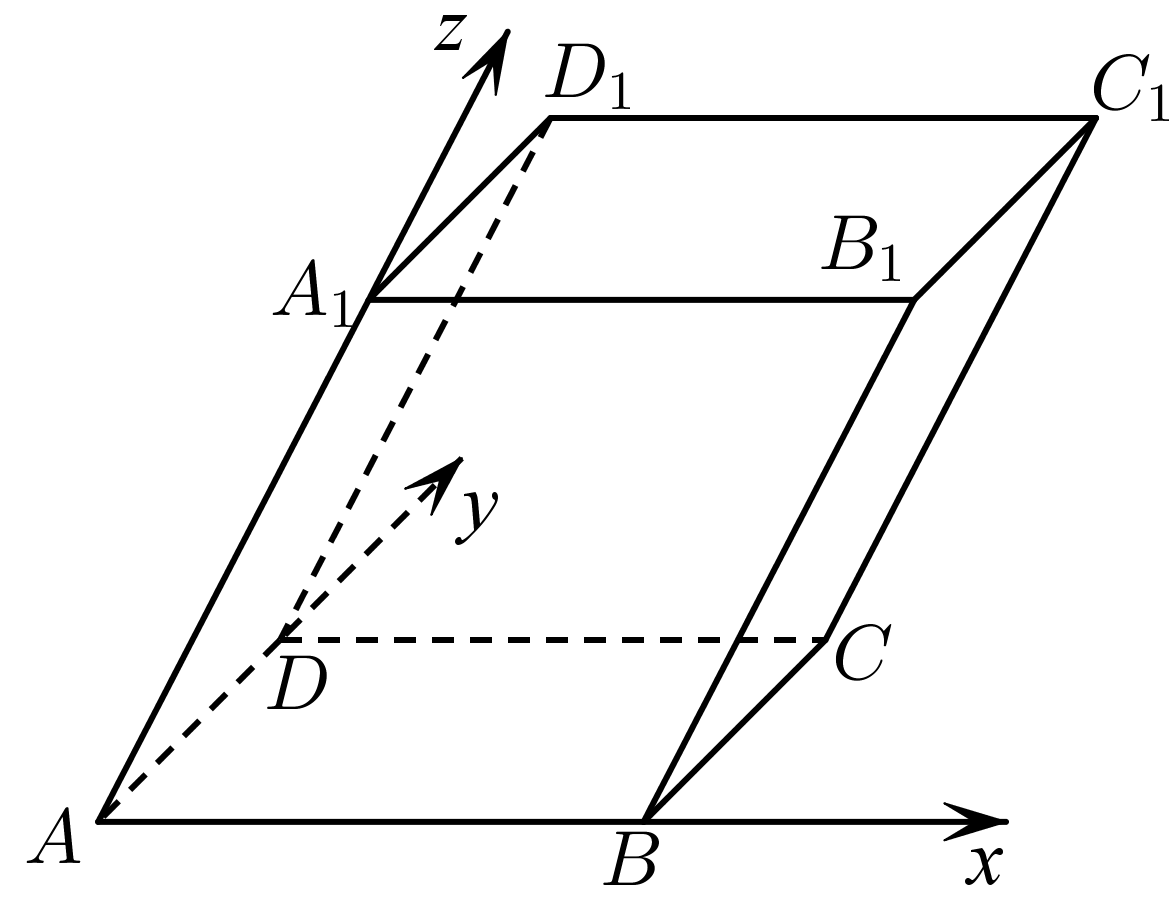
\includegraphics[width=58.0mm]{figs/js_image12.png}}\par\vspace{-1.0mm}\penalty-50
\lxopt{①若\(\overrightarrow{BE}=\overrightarrow{EB_1}\)，求向量\(\overrightarrow{ED_1}\)的斜\(60^{\circ}\)坐标；②若\(\overrightarrow{AM}=[2,t,0]\)，且\(\overrightarrow{AM}\perp\overrightarrow{AC_1}\)，求\(|AM|\)．}
\xiexwei{16mm}
\begin{ansblock}[练-课时05-14]
% ans:练-课时05-14
\setlength{\anshang}{7.6mm}% 题14 起双位档（照答案册同值，块内局部）
\ansitem{14}{(1)\([0,3,5]\)；①\(\left[-2,2,\dfrac{3}{2}\right]\)；②\(|AM|=2\)}
\end{ansblock}

\dangbadge{思}{维}{探}{索}

\tihao{15}\zu{存在性判定×值域·解答（E15 改造底）} \tieside{难}已知向量\(\overrightarrow{a}=(1,2,0)\)，\(\overrightarrow{b}=(0,1,2)\)．对实数\(m\)，记\(\overrightarrow{u}=\overrightarrow{a}+m\overrightarrow{b}\)，\(\overrightarrow{v}=m\overrightarrow{a}-\overrightarrow{b}\)．
\lxopt{(1)判断是否存在实数\(m\)使得\(\overrightarrow{u}\perp\overrightarrow{v}\)？若存在，求出所有这样的\(m\)；若不存在，说明理由；}
\lxopt{(2)判断是否存在实数\(m\)使得\(\overrightarrow{u}\parallel\overrightarrow{v}\)？若存在，求出所有这样的\(m\)；若不存在，说明理由；}
\lxopt{(3)设\(\theta=\langle\overrightarrow{u},\overrightarrow{v}\rangle\)（向量\(\overrightarrow{u}\)与\(\overrightarrow{v}\)的夹角）．求\(\cos\theta\)的取值范围，并说明两端等号能否取得．}
\xiexwei{16mm}
\begin{ansblock}[练-课时05-15]
% ans:练-课时05-15
\setlength{\anshang}{7.6mm}% 题15 起双位档（照答案册同值，块内局部）
\ansitem{15}{(1)\(m=\pm 1\)；(2)不存在；(3)\(\left[-\dfrac{2}{5},\dfrac{2}{5}\right)\)}
\end{ansblock}

\tihao{16}\zu{双动点定距×数量积范围·解答（T7 改造底）} \tieside{难}在棱长为\(2\)的正方体\(ABCD\text{-}\penalty100 A_1B_1C_1D_1\)中，以\(A\)为原点，\(\overrightarrow{AB}\)、\(\overrightarrow{AD}\)、\(\overrightarrow{AA_1}\)的方向为\(x\)轴、\(y\)轴、\(z\)轴正方向建立空间直角坐标系．点\(P\)在棱\(A_1B_1\)上，\(\overrightarrow{A_1P}=\lambda\overrightarrow{A_1B_1}\)（\(0\leq\lambda\leq1\)）；点\(Q\)在棱\(B_1C_1\)上，\(\overrightarrow{B_1Q}=\mu\overrightarrow{B_1C_1}\)（\(0\leq\mu\leq1\)）．已知\(|\overrightarrow{PQ}|=1\)．
\lxopt{(1)写出\(P\)、\(Q\)的坐标，求\(\lambda\)与\(\mu\)满足的关系式，并求\(\lambda\)的取值范围；}
\lxopt{(2)求\(\overrightarrow{PQ}\cdot\overrightarrow{CA_1}\)的取值范围．}
\xiexwei{16mm}
\begin{ansblock}[练-课时05-16]
% ans:练-课时05-16
\setlength{\anshang}{7.6mm}% 题16 起双位档（照答案册同值，块内局部）
\ansitem{16}{(1)\((1-\lambda)^{2}+\mu^{2}=\dfrac{1}{4}\)，\(\lambda\in\left[\dfrac{1}{2},1\right]\)；(2)\([-2\sqrt{2},-2]\)}
\end{ansblock}

\end{multicols}

\tailfill
\end{document}
